% Options for packages loaded elsewhere
\PassOptionsToPackage{unicode}{hyperref}
\PassOptionsToPackage{hyphens}{url}
\PassOptionsToPackage{dvipsnames,svgnames,x11names}{xcolor}
%
\documentclass[
  number,
  3p]{elsarticle}

\usepackage{amsmath,amssymb}
\usepackage{iftex}
\ifPDFTeX
  \usepackage[T1]{fontenc}
  \usepackage[utf8]{inputenc}
  \usepackage{textcomp} % provide euro and other symbols
\else % if luatex or xetex
  \usepackage{unicode-math}
  \defaultfontfeatures{Scale=MatchLowercase}
  \defaultfontfeatures[\rmfamily]{Ligatures=TeX,Scale=1}
\fi
\usepackage{lmodern}
\ifPDFTeX\else  
    % xetex/luatex font selection
\fi
% Use upquote if available, for straight quotes in verbatim environments
\IfFileExists{upquote.sty}{\usepackage{upquote}}{}
\IfFileExists{microtype.sty}{% use microtype if available
  \usepackage[]{microtype}
  \UseMicrotypeSet[protrusion]{basicmath} % disable protrusion for tt fonts
}{}
\makeatletter
\@ifundefined{KOMAClassName}{% if non-KOMA class
  \IfFileExists{parskip.sty}{%
    \usepackage{parskip}
  }{% else
    \setlength{\parindent}{0pt}
    \setlength{\parskip}{6pt plus 2pt minus 1pt}}
}{% if KOMA class
  \KOMAoptions{parskip=half}}
\makeatother
\usepackage{xcolor}
\setlength{\emergencystretch}{3em} % prevent overfull lines
\setcounter{secnumdepth}{5}
% Make \paragraph and \subparagraph free-standing
\ifx\paragraph\undefined\else
  \let\oldparagraph\paragraph
  \renewcommand{\paragraph}[1]{\oldparagraph{#1}\mbox{}}
\fi
\ifx\subparagraph\undefined\else
  \let\oldsubparagraph\subparagraph
  \renewcommand{\subparagraph}[1]{\oldsubparagraph{#1}\mbox{}}
\fi


\providecommand{\tightlist}{%
  \setlength{\itemsep}{0pt}\setlength{\parskip}{0pt}}\usepackage{longtable,booktabs,array}
\usepackage{calc} % for calculating minipage widths
% Correct order of tables after \paragraph or \subparagraph
\usepackage{etoolbox}
\makeatletter
\patchcmd\longtable{\par}{\if@noskipsec\mbox{}\fi\par}{}{}
\makeatother
% Allow footnotes in longtable head/foot
\IfFileExists{footnotehyper.sty}{\usepackage{footnotehyper}}{\usepackage{footnote}}
\makesavenoteenv{longtable}
\usepackage{graphicx}
\makeatletter
\def\maxwidth{\ifdim\Gin@nat@width>\linewidth\linewidth\else\Gin@nat@width\fi}
\def\maxheight{\ifdim\Gin@nat@height>\textheight\textheight\else\Gin@nat@height\fi}
\makeatother
% Scale images if necessary, so that they will not overflow the page
% margins by default, and it is still possible to overwrite the defaults
% using explicit options in \includegraphics[width, height, ...]{}
\setkeys{Gin}{width=\maxwidth,height=\maxheight,keepaspectratio}
% Set default figure placement to htbp
\makeatletter
\def\fps@figure{htbp}
\makeatother

\makeatletter
\makeatother
\makeatletter
\makeatother
\makeatletter
\@ifpackageloaded{caption}{}{\usepackage{caption}}
\AtBeginDocument{%
\ifdefined\contentsname
  \renewcommand*\contentsname{Table of contents}
\else
  \newcommand\contentsname{Table of contents}
\fi
\ifdefined\listfigurename
  \renewcommand*\listfigurename{List of Figures}
\else
  \newcommand\listfigurename{List of Figures}
\fi
\ifdefined\listtablename
  \renewcommand*\listtablename{List of Tables}
\else
  \newcommand\listtablename{List of Tables}
\fi
\ifdefined\figurename
  \renewcommand*\figurename{Figure}
\else
  \newcommand\figurename{Figure}
\fi
\ifdefined\tablename
  \renewcommand*\tablename{Table}
\else
  \newcommand\tablename{Table}
\fi
}
\@ifpackageloaded{float}{}{\usepackage{float}}
\floatstyle{ruled}
\@ifundefined{c@chapter}{\newfloat{codelisting}{h}{lop}}{\newfloat{codelisting}{h}{lop}[chapter]}
\floatname{codelisting}{Listing}
\newcommand*\listoflistings{\listof{codelisting}{List of Listings}}
\makeatother
\makeatletter
\@ifpackageloaded{caption}{}{\usepackage{caption}}
\@ifpackageloaded{subcaption}{}{\usepackage{subcaption}}
\makeatother
\makeatletter
\@ifpackageloaded{tcolorbox}{}{\usepackage[skins,breakable]{tcolorbox}}
\makeatother
\makeatletter
\@ifundefined{shadecolor}{\definecolor{shadecolor}{rgb}{.97, .97, .97}}
\makeatother
\makeatletter
\makeatother
\makeatletter
\makeatother
\journal{Science eLetter}
\ifLuaTeX
  \usepackage{selnolig}  % disable illegal ligatures
\fi
\usepackage[]{natbib}
\bibliographystyle{elsarticle-num}
\IfFileExists{bookmark.sty}{\usepackage{bookmark}}{\usepackage{hyperref}}
\IfFileExists{xurl.sty}{\usepackage{xurl}}{} % add URL line breaks if available
\urlstyle{same} % disable monospaced font for URLs
\hypersetup{
  pdftitle={Response to West et al.~(2023)},
  pdfauthor={Hugh A. Graham; Andrew M. Cunliffe; Edward T.A. Mitchard; Javier Ruiz Ramos; Leonardo Sáenz; David F.R.P. Burslem; Christopher D. Philipson},
  colorlinks=true,
  linkcolor={blue},
  filecolor={Maroon},
  citecolor={Blue},
  urlcolor={Blue},
  pdfcreator={LaTeX via pandoc}}

\setlength{\parindent}{6pt}
\begin{document}

\begin{frontmatter}
\title{Response to West et al.~(2023)}
\author[1,2]{Hugh A. Graham%
\corref{cor1}%
}
 \ead{hugh.graham@permianglobal.com} 
\author[2]{Andrew M. Cunliffe%
%
}

\author[3]{Edward T.A. Mitchard%
%
}

\author[1]{Javier Ruiz Ramos%
%
}

\author[1]{Leonardo Sáenz%
%
}

\author[4]{David F.R.P. Burslem%
%
}

\author[1]{Christopher D. Philipson%
\corref{cor1}%
}
 \ead{christopher.philipson@permianglobal.com} 

\affiliation[1]{organization={Permian Global Research
Ltd.},addressline={3 Cavendish Square},city={London},postcode={W1G
0LB},postcodesep={}}
\affiliation[2]{organization={University of Exeter, Geography, Faculty
of Environment, Science and Economy},,postcodesep={}}
\affiliation[3]{organization={Space Intelligence Ltd.},addressline={93
George Street},city={Edinburgh},postcode={EH2 3ES},postcodesep={}}
\affiliation[4]{organization={University of Aberdeen, School of
Biological Sciences},city={Aberdeen},postcode={AB24 3UU},postcodesep={}}

\cortext[cor1]{Corresponding author}







        





\end{frontmatter}
    \ifdefined\Shaded\renewenvironment{Shaded}{\begin{tcolorbox}[borderline west={3pt}{0pt}{shadecolor}, boxrule=0pt, frame hidden, enhanced, sharp corners, breakable, interior hidden]}{\end{tcolorbox}}\fi

Avoided deforestation conservation projects necessitate comparisons
between observations in protected forests and what-would-have-happened
if the project did not exist (often referred to as the baseline, or
counterfactual scenario) \citep{balmford_realizing_2023}. Nevertheless,
it is imperative that forest carbon projects deliver the carbon emission
reductions they report, and there are various methods that can be used
to estimate these counterfactual scenarios. West et al.
\citep{west_action_2023} used the synthetic control method to choose
pools of controls with similar covariate structure to \emph{avoided
unplanned deforestation conservation project} areas; they do not
consider other methodologies such as \emph{planned avoided
deforestation}, or \emph{improved forest management}. Synthetic controls
were calculated from the mean deforestation rate of pools, weighted by
covariate similarity with the project. We agree that the synthetic
control method could potentially improve the evaluation of forest carbon
projects. However, synthetic controls are also vulnerable to ``gaming''
or bias through inappropriate donor pool design/sampling and such
econometric statistical methods require further context-specific
refinement \citep{balmford_realizing_2023} before they can improve upon
existing approaches.

West et al. \citep{west_action_2023} claim that most forest carbon
projects overestimate avoided deforestation or do not significantly
reduce deforestation. These conclusions are poorly supported by their
analysis because:

\begin{itemize}
\item
  The implemented synthetic control approach can suffer from bias
  \citep{abadie_using_2021} due to substantial and incompatible
  differences between deforestation drivers, forest type and
  (bio)geography that are not adequately captured by the structure of
  covariates that are used to form the synthetic control. Important
  covariates are ignored, such as distance to roads and rivers
  \citep{laurance_roads_2017, barber_roads_2014}, fire risk
  \citep{amador-jimenez_unintended_2020}, or indicators of forest
  structure \citep{duncanson_aboveground_2022} that predict biomass,
  timber value and logging effort. Using the authors' code, we extracted
  the locations of controls used to create the synthetic control for
  project-856 (Figure~\ref{fig-map}), located in Colombia's
  Pacific-montane-forest. No weighted donors were in the same political
  jurisdiction or ecoregion as the project and the highest weighted
  donor (0.46) was in the Amazon, 900 km away. We have also attempted to
  reproduce the synthetic controls for all considered project areas;
  interactive maps of these locations are presented at
  https://permian-global-research.github.io/science-letter-west-et-al/.
\item
  Calculations derived from Global Forest Change (GFC)
  \citep{hansen_quantification_2010} inherit known sensitivity and
  accuracy issues
  \citep{kinnebrew_biases_2022, galiatsatos_assessment_2020}. It is
  inappropriate to compare GFC-based calculations with those reported by
  projects, which are better calibrated for local contexts, because
  meaningful comparisons require deforestation rates to be derived using
  identical methods. Further, it is accepted that GFC is inappropriate
  for site-level deforestation assessment, in isolation
  \citep{galiatsatos_assessment_2020, bos_global_2019}.
\item
  West et al. \citep{west_action_2023} do not demonstrate that synthetic
  control counterfactuals are more accurate than project methods,
  undermining their ability to interpret differences between the
  synthetic control and project-reported deforestation rates.
\end{itemize}

\begin{figure}[H]

{\centering 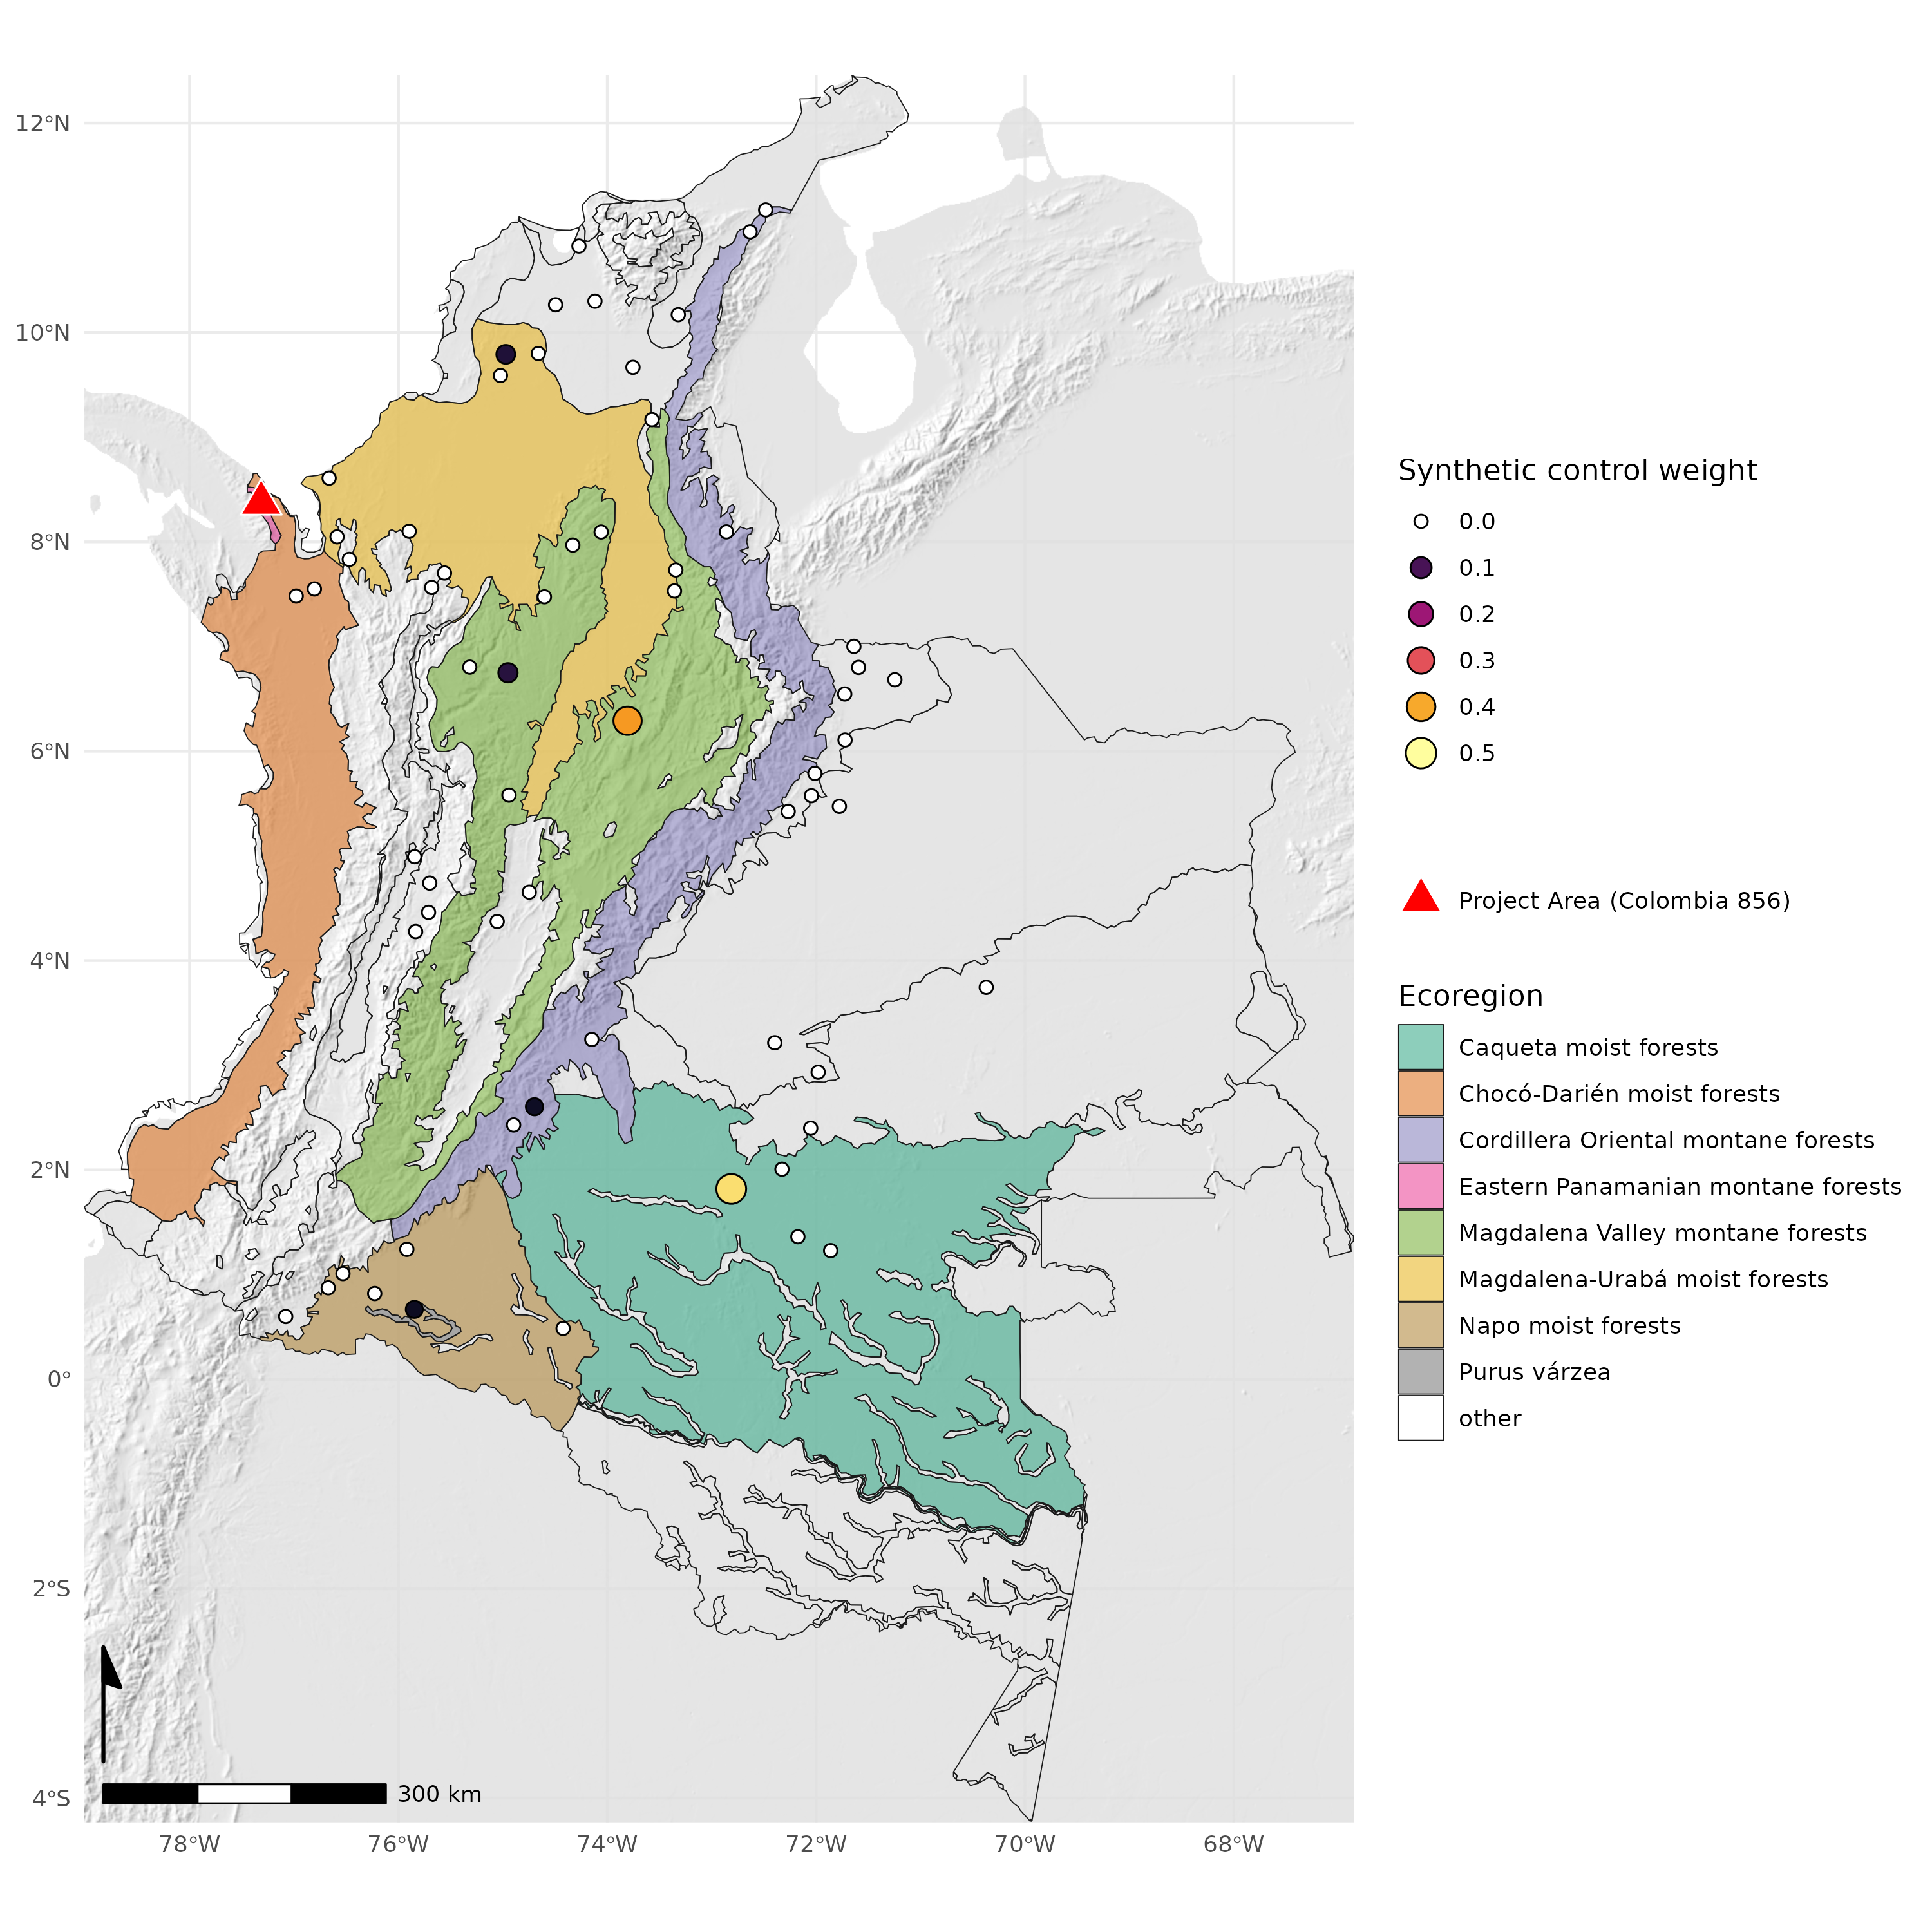
\includegraphics{figures/colombia_856_donors.png}

}

\caption{\label{fig-map}Map of the donor pool and their weighted
contribution to the synthetic control for Project-856. The project is
located to the north of Colombia's Choco Department (political
jurisdiction), in the Darien Mountain range and comprises a transition
from lowland to montane rainforest. Also presented are ecoregions
\citep{dinerstein_ecoregion-based_2017} that intersect weighted donors.
Two donors form more than 84\% of the synthetic control, and no weighted
donors were in the same ecoregion as the project with the highest
weighted donor being 900 km away, in the Amazon. Project-856 was
selected because it was the only one where fully reproducible code was
made available. To see interactive maps of this and all other projects
please see
\url{https://permian-global-research.github.io/science-letter-west-et-al/}.
Elevation data from https://registry.opendata.aws/terrain-tiles.}

\end{figure}

The adoption of econometric methods to evaluate the efficacy of
voluntary carbon projects is an important development in the field
\citep{balmford_realizing_2023}, yet these methods need improvement.
Critically, the drivers of deforestation are complex and highly variable
across space and time. We believe that there is a need to more carefully
consider the connections between spatial and econometric statistical
techniques, in the context of remote sensing, to maximise the accuracy
and utility of these methods \citep{garcia_conservation_2022}.

No method of reconstructing a counterfactual can claim to represent
absolute truth. In order to improve the evaluation of avoided
deforestation conservation projects, one potential way forward could be
to adopt a simulation framework to benchmark the efficacy of synthetic
controls alongside alternative methods. Simulations to reconstruct
counterfactuals on non-project areas will provide quantitative metrics
for counterfactual reconstruction accuracy. We hope this letter will
stimulate further discussion on this topic and encourage the development
and adoption of improved inference methods in voluntary carbon projects.

\hypertarget{references}{%
\section{References}\label{references}}

\renewcommand{\bibsection}{}
\bibliography{bibliography.bib}




\end{document}
